\documentclass[12pt]{article}

\usepackage{fancyhdr} % Required for custom headers
\usepackage{float}
\usepackage{lastpage} % Required to determine the last page for the footer
\usepackage{extramarks} % Required for headers and footers
\usepackage{graphicx} % Required to insert images
\usepackage{amssymb}
\usepackage{enumerate}
\usepackage{svg}
\usepackage{caption}
\usepackage{subfig}

% Margins
\topmargin=-.5in
\evensidemargin=0in
\oddsidemargin=0in
\textwidth=6.5in
\textheight=9in
\headsep=0.25in

\DeclareGraphicsExtensions{.jpg,.png,.svg}

\newcommand{\tab}{\hspace*{2em}}

\title{Combined Task and Motion Planner through an Interface Layer}
\author{Alex Gutierrez (ragtz@mit.edu), Bianca Homberg (bhomberg@mit.edu), \\and Veronica Lane (vmlane@mit.edu)}


%% ONE SENTENCE PER LINE TO MAKE THIS WORK NICELY IN GIT

\begin{document}

\maketitle

\section{Introduction}

In order to achieve high level goals a robot must combine task and motion planning. 
A robot uses task planning to determine its long term strategy and motion planning to determine the movements it  will execute to achieve the task. 
Effectively combining task and motion planning is an open research problem. 
We implemented an interface between the motion and task planning based on that outlined in [1]. 
Our system uses off-the-shelf task and motion planners and makes few assumptions about their implementation.
 
An alternative approach to developing an interface between the task and motion planner is for the task planner to discretize the geometric state space. 
However, the number of required discretizations to solve the problem is generally very large and results in extremely large or infeasible problems. 
An interface allows the task planner state space to use an abstract state space which ignores geometry. 
The interface layer translates geometric constraints and passes them to the task planner.

\section{Problem Statement}

In robotics, it is often necessary to create a plan for a series of motions of the robot in order to achieve some high level objective.
In order to find a task plan which is actually feasible, the task planner must have some knowledge of the geometry of the world.
Without knowledge of the actual spatial configurations of objects in the world, the task planner would create plans that could not complete some actions, due to infeasible motion plans from blocking objects or interference between the robot and the environment.

The high level problem this implementation addresses is to create a combined task and motion planner, following that presented in [1].  
This approach allows the motion planner to give information to the task planner and keeps continuous variables continuous, rather than discretizing.  
This prevents a combinatorial explosion of the state space that the task planner needs to search over.

The main contribution of this implementation is an interface layer.  
This interface layer is designed to be planner-independent: that is, it can work with any motion planner and task planner, so long as the outputs from each are conformed to the interface specification.  
The interface layer interleaves calls between the task planner and the motion planner, using geometric feasibility determined through the motion planner to affect the state given to the task planner to plan from.




\section{High Level Approach}

The interface layer starts by asking the task planner to generate a high level plan and has the motion planner instantiate motion plans corresponding to each action.  
When it's not possible to generate a motion plan, the interface layer determines what geometric constraints are causing the problem and relays this back to the task planner.  
Then, the task planner replans from that state and the process continues.  
When necessary, backtracking occurs.
 
At start time, the task planner is given a PDDL domain specifying the different actions that are feasible along with their preconditions and postconditions.  
For individual calls to the task planner, the interface layer takes an internal `state' variable, converts it to PDDL format, and sends it along to be solved.  
The task planner responds with a high level plan or a notification that finding a plan failed.  
If finding a plan failed, the interface layer begins backtracking.  
If a high level plan is found, the interface layer begins searching for refinements of each action as a motion plan.

On each call to the motion planner, the interface layer provides the motion planner with the intended action, the world state, and a pose or set of poses  
corresponding to sub-parts of the action. These poses are randomly generated for each action by a pose generator within the interface layer. 
If it is possible to perform the action using the intermediary poses specified, the motion plan returns the trajectory and the updated world state.  
If not, it returns an error message.

If the motion plan does not succeed, a variety of poses are tried.  
Again, poses are generated randomly from a pose generator.  
If no poses are successful, the interface layer determines what is blocking the motion plan from succeeding by removing objects from the environment until a feasible motion plan is found.  
If still no feasible motion plan is found, backtracking is required.  
If a feasible motion plan is found with some subset of objects removed, then that information is relayed back to the task planner after the PDDL state is appropriately updated.
This update adds predicates corresponding to the object obstructions, and the task planner is asked to replan starting from the step where we failed to find a motion plan. This whole process continues until a feasible motion plan has been found.  


\subsection{Simple Example Walkthrough}

\begin{figure}[t]
\centering
\def\svgwidth{0.5\textwidth}
\input{figures/walkthrough.pdf_tex}
\caption{Walkthrough Example. The goal is for the red block to be on surface S.\label{fig:walkthrough}}
\end{figure}

In this environment, we have two objects, blocks 1 and 2, and our goal is to put block 1 into area S.  
However, we cannot pick up block 1 directly since the walls and block 2 surround it.  
Here we walk through the steps the interface layer takes when solving this problem in order to explain the details of the interface layer's construction.

\begin{enumerate}[i.]

\item Call the task planner to create a high level plan.  
In this case, the task planner doesn't yet know that block 2 is blocking block 1, so the plan is simply:

\begin{enumerate}[1.]
\item PICKUP BLOCK1 with GRIPPER

\item PUTDOWN BLOCK1 on SURFACE S
\end{enumerate}

\item Next step is to call the motion planner to try and find a trajectory corresponding to each of these actions.  
In this case, the motion planner fails to find a motion plan for step 1.  

\item The interface layer goes through removing objects to try to find what was causing the error for that action.  
The interface layer discovers that if it removes block 2, then the motion plan can be created just fine, so block 2 must be obstructing the path.

\item We add a predicate corresponding to BLOCK2 OBSTRUCTS BLOCK1 to the planner's state.

\item Now, we try to find a new high level plan.  
Since block 2 is obstructing block 1, we can't pick up block 1 directly, so the task planner realizes it needs to move block 2 first before moving block 1. 
The new plan it creates is:

\begin{enumerate}[1.]
\item PICKUP BLOCK2 	with GRIPPER
\item PUTDOWN BLOCK2 on SURFACE S
\item PICKUP BLOCK1 with GRIPPER
\item PUTDOWN BLOCK1 on SURFACE S
\end{enumerate}

\item Now, we again go to the motion planner and try to find a motion plan corresponding to every action.
In this case, there are no more obstructions, so the process works!

\item Ultimately, the algorithm returns the high level plan in conjunction with a motion plan trajectory for every step of the high level plan.

\end{enumerate}

\section{Technical Details}

In this section, we discuss the key insight of the original paper: the ability to avoid discretization by representing continuous variables symbolically via references.  
We also discuss the pose generators which propose real-world instantiations of these references.  
Finally, we walk through the algorithm in detail.

\subsection{Representing Continuous Variables Symbolically}

One of the key insights of this paper is that continuous variables can be referenced symbolically in the task planner within the PDDL domain.  
For instance, consider the pose of the robot: this is a continuous, geometric state.  However, the task planner only keeps track of poses symbolically.  
The task planner knows that there is some GPFG\_obj\_1 -- a Gripper Pose For Grasping -- for object 1, and it doesn't really care what that pose is, so long as it exists.  
The task planner reasons over a variety of these symbolic variables, corresponding to poses and trajectories.  
The motion planner and pose generators take these symbolic variables and associate them with corresponding real locations and motions in the world.  
This is the key insight which allows the task planner to reason about continuous variables without discretizing.  

We will follow [1] in using manipulation as an example environment.  For any planning domain with some continuous variables and some discrete variables, it will be possible to transform the continuous variables to discrete symbolic references to continuous positions.  For this example, we talk through the PICKUP action for a simple manipulator; the PUTDOWN action is analagous.


\vspace{10pt}

$PICKUP(obj_1, gripper, pose_1, pose_2, traj)$

$\; precon \; EMPTY(gripper), ROBOTAT(pose_1), $

$\; \; \;\; \; \; ISGPFG(pose_2, obj), ISMP(traj, pose_1, pose_2), $

$\; \; \; \; \; \;\forall obj' \neg OBSTRUCTS(obj', traj, obj_1)$

$\; effect \; IN(obj_1, gripper), \neg EMPTY(gripper), $

$\; \; \;\; \; \; \forall obj', traj' \neg OBSTRUCTS(obj_1, traj', obj'), $

$\; \; \; \; \; \;\forall obj' traj', tloc' \neg PDOBSTRUCTS(obj_1, traj', obj', tloc')$

\vspace{10pt}

Here, we have three continuous variables that we represent symbolically: $traj$, for each of the trajectories, and $pose_1$ and $pose_2$, representing start and end locations for the robot's gripper.
The preconditions and effects can also iterate over all of these symbolic variables, allowing us to mark that a picked up object doesn't obstruct any other objects, etc. 
We have various predicates which describe different things about both the discrete variables and the continuous variables.

\vspace{10pt}

$EMPTY(gripper)$ -- gripper is empty and thus available to hold a block.

$ROBOTAT(pose_1)$ -- robot pose,  $pose_1$ is a symbolic reference to a continuous variable.

$ISGPFG(pose, obj)$ -- $pose$ is a Gripper Pose For Grasping (GPFG) an object $obj$.

$ISMP(traj, pose_1, pose_2)$ -- $traj$ is a motion plan from $pose_1$ to $pose_2$.

$OBSTRUCTS(obj_1, traj, obj_2)$ -- $obj_1$ blocks $obj_2$ from being picked up along $traj$.

$PDOBSTRUCTS(obj_1, traj, obj_2, tloc)$ -- $obj_1$ blocks $obj_2$ from placement at $tloc$ along $traj$.

$IN(obj_1, gripper)$ -- $obj_1$ currently grasped by $gripper$.

\vspace{10pt}

How do we come up with all of these symbolic references?  
We create as many as we need.  
In this case, we need to have a pose where we can pick up each object and put each object down.  
Neither the interface layer nor the task planner know what the poses correspond to in the real world.
The pose generators instantiate specific poses which the motion planner verifies or discounts if it doesn't work.
Similarly, we have one trajectory for each potential pair of poses.  
However, since the trajectory isn't actually used in any of the effects, we actually can ignore it entirely -- it doesn't change the high level plan and the interface layer will still know to have the motion planner create the relevant trajectories. 
So to make the plan more efficient, we actually cut out the $ISMP$ predicate and all references to trajectories.

How do we pass geometric information from the environment back to the task planner?  
We do this via the $OBSTRUCTS$ and $PDOBSTRUCTS$ predicates.  
These tell the task planner that certain objects are blocking motions related to other objects.  
This allows the task planner to have the robot first move the blocking objects so it can get to the other objects.


\subsection{Pose Generators}

When the pose generator is called by the interface layer, it generates a set of random poses for each action. Each pose is made up of a set of waypoints. For example for the PICKUP action, it generates the following waypoints: near the cylinder and pointing towards it, touching the cylinder, lifting the cylinder, and a standard home position. It passes one pose to the interface layer at a time.  if none of the poses are feasible, the interface layer backtracks and resets the pose generator. The TryRefine method of the interface layer attempts to generate a feasible motion plan between each pose.  The motion planner is called to create this motion plan, including motion plans between waypoints.

\subsection{Main Interface Layer}

\begin{figure}[t]
\centering
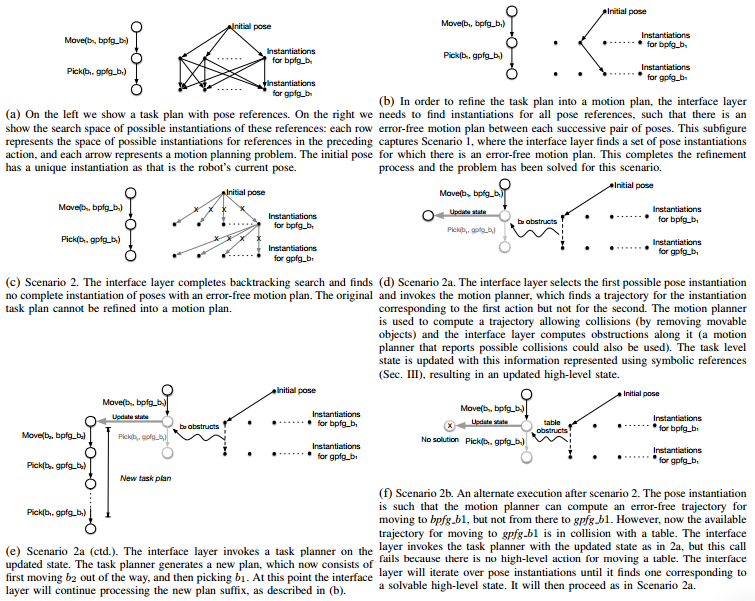
\includegraphics[width=\textwidth]{figures/figure4.png}
\caption{Illustration of the interface layer’s refinement process. Action arguments have been abbreviated. Taken from [1]
\label{fig:figure4}}
\end{figure}

This figure (Fig. \ref{fig:figure4}), included with text from [1], explains the flow of control of the interface layer through a variety of situations, including more than the simple case covers.  
The subfigures in this diagram explain on a high level the different steps the interface layer takes when solving a problem.  
The subfigure a shows the motion planner's backtracking search when trying to instantiate motions for each of the high level actions.  
Subfigure b shows the first possible scenario, where the backtracking search succeeds.  Subfigure c shows a second possible scenario, where the backtracking search doesn't succeed.  
There are multiple options of what can happen within this scenario: subfigure d shows an option where they determine that the block2 obstructs the trajectory.  
This triggers the behavior discussed earlier, where the state is updated for the task planner.  
Subfigure e shows the new task plan after replanning occurs.  
After this, the interface layer will repeat the process of attempting to refine this new plan.  
Subfigure f shows an alternative option, where the blocking object is determined to be the table, which is not movable.  
Then, the state is updated as before and the task planner is called, but no solution is found, so backtracking occurs.

\subsubsection{Algorithm Improvements}

The original version of the algorithm, as shown in (Fig. \ref{fig:algorithms}), only attempts to find partial trajectories when it replans partway through the procedure.  Our algorithm has a slight modification. Every time a new partial plan is generated, we first try to fill it completely using backtracking search before giving up and resorting to the partial trajectory finding.  In some scenarios, some poses will not work but others will, so it is better to try to make the simplest possible plan work before giving up and making the high level plan more complicated.  In our manipulation example, this turns into trying to pick up blocks from all angles before giving up and assuming they must be blocked by something.  An analysis of the benefits of this approach are outlined in the benchmarking section.  

\subsubsection{Algorithm 1}

\begin{figure}[t]
	\centering
	\subfloat{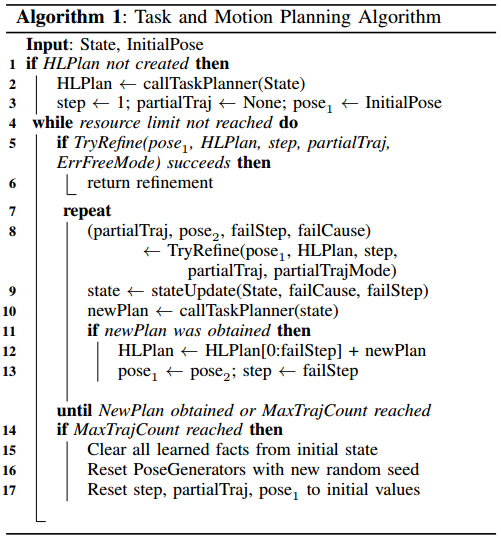
\includegraphics[width=.45\linewidth]{figures/algorithm1}}
	\qquad
	\subfloat{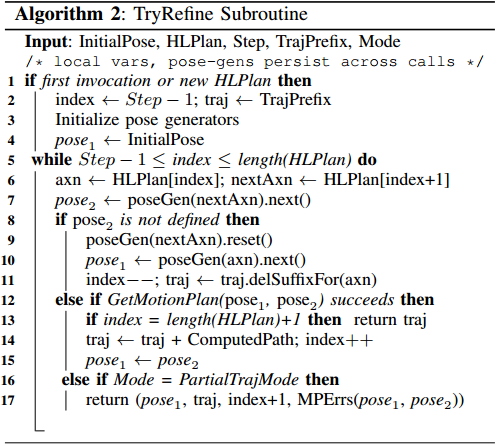
\includegraphics[width=.45\linewidth]{figures/algorithm2}}
	\caption{Taken from[1]\label{fig:algorithms}}
\end{figure}

The outer loop of the algorithm interfaces with the high level task planner.  
We start with an initial state where no objects obstruct any motions.  
From there, we look for a high level plan.  
If the problem is not solvable even without any obstructions from the environment, then the problem is unsolvable and we immediately return that information.  
If we do succeed at finding a high level task plan, we begin the process of attempting to find a motion corresponding to each action.

First, we start by attempting to find a full refinement of the whole plan, calling the TryRefine subroutine in error-free mode.  
If that succeeds, then we return the plan.  

If that doesn't succeed, we find a partial trajectory that goes as far as it can by calling the TryRefine subroutine in partial trajectory mode.  
This function returns a partial trajectory along with the step where it failed and the determined cause for failure.  
Then, we update the state based on the actions up until that point and add in the obstructing obstacles corresponding to the failure.  
Now, we attempt to find a new high level plan, and iterate.  

If we fail to find a new high level plan at any point, we re-run the TryRefine subroutine on the original high level plan from the previous step.  
Since the TryRefine subroutine has randomization from pose generators, re-running it may yield a better solution. 

We have several checks where, if we fail to find a solution, we clear all of our information and start over.  Due to the randomization of the pose generators, we may make better choices during subsequent iterations.  

The original version of the algorithm, as shown in \ref{fig:algorithms}, only attempts to find partial trajectories when it replans partway through the procedure.  For our version of the algorithm, every time a new partial plan is generated, we first try to fill it completely using backtracking search (calling TryRefine in error-free mode) before giving up and resorting to the partial trajectory finding.  

\subsubsection{Algorithm 2}


In the TryRefine subroutine, the interface layer attempts to find motion plans corresponding to the various actions.  
It has two modes: error free and partial trajectory.  
In error free mode, it performs backtracking search to try to find a full plan from start to finish.  
The backtracking search is over possible pose instantiations: since some poses may be infeasible and since previous choices may affect future choices, the backtracking search iterates over all possible poses in order to find a full solution if a full solution exists.  

In partial trajectory mode, TryRefine goes as far as it can, but when it finds an infeasible motion plan for some action, it returns the step at which it failed.  
In addition to returning the failed step, it returns the cause of the errors.  
The function MPErrs removes various objects from the environment until it find a plan which succeeds.  
It then marks all of those objects which were removed as blocking objects.

To find the blocking objects, we start by iterating through a randomized list of the objects.  We continue removing objects until we find a successful motion plan.  
We will eventually find a successful motion plan since if there are no other objects in the world, the motion should succeed.  
After we find this possible list of removed objects, we iterate through all of the objects we removed.  
We attempt to add these objects in one by one, leaving added in all of those which don't obstruct our found motion plan.  
This leaves us with a local minimum of removed objects: it may be possible to find another smaller set of objects that, if removed, allow a valid motion plan.  
However, for this set of this set of objects, no object can be added back in without obstructing the motion plan.

As described above in Algorithm 1, once the list of blocking objects is returned, the interface layer updates the state and attempts to replan from there.


\section{Benchmarking}
\subsection{Testing}
\begin{figure}[t]
\centering
\def\svgwidth{0.5\textwidth}
\input{figures/smallEnv.pdf_tex}
\caption{Small Environment Test Example. The goal was for the blue blocks to be on surface I and the red blocks to be on surface S.\label{fig:smallEnv}}
\end{figure}
We generated a set of small-scale tests to check the correctness of the interface layer. ref{fig-smallTest} Each test had three to four blocks initially placed on one or two surfaces. Some blocks were surrounded on 3 sides and others on all sides by walls and blocks. For blocks surrounded on 3 sides, the interface layer had to find the pose that picked up the block in the correct direction. For blocks surrounded on all sides, the interface layer needed to generate actions to move blocks in the way.

\subsection{Procedure}
\begin{figure}[t]
\centering
\def\svgwidth{\textwidth}
\input{figures/benchmarks.pdf_tex}
\caption{Benchmarking Test Examples. The goal was to move the green block to another surface.\label{fig:benchmark}}

\end{figure}

We performed a variety of benchmarking tests to measure the performance of the interface. We measured the performance of each test by the number of calls to both the task planner and motion planner and the runtime. ref{table-benchmarkTable}
The difficulty of a benchmark increased as the total number \textit{obstructions} increased. The total number of obstructions was counted by summing the number of directions around each block that were obstructed. For the ordinal directions, a neighboring block in any one of three locations obstructs the direction. For example, a neighboring block above, to the right or to the top right corner of a block obstructs the northeast direction of the block. Furthermore, as the number of blocks for a particular grid shape increased, the test difficulty increased, since the total number of obstructions increased.

\subsection{Results}
\begin{figure}[t]
	\centering
	\subfloat{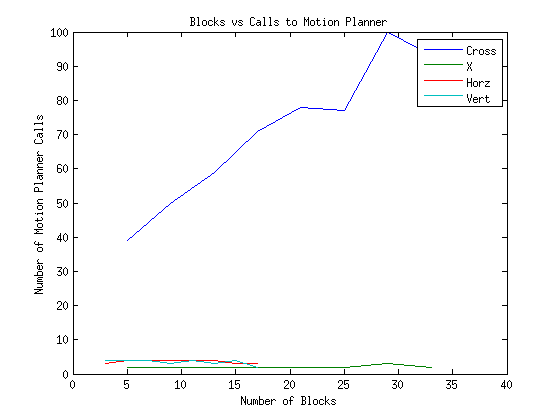
\includegraphics[width=.45\linewidth]{figures/bvm}}
	\qquad
	\subfloat{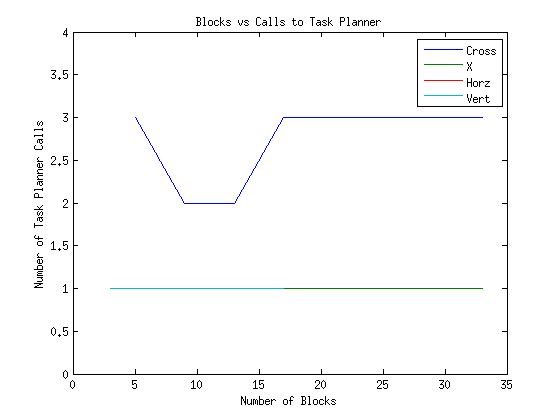
\includegraphics[width=.45\linewidth]{figures/bvt}}
	\qquad
	\subfloat{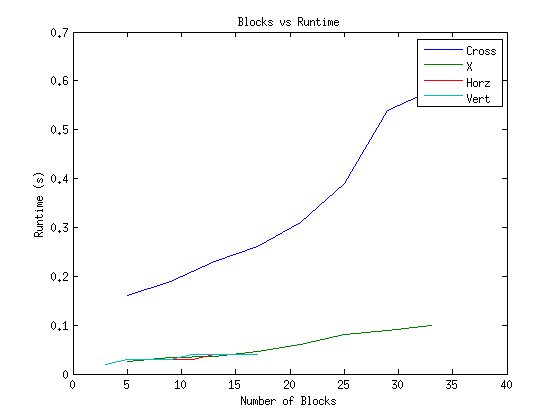
\includegraphics[width=.45\linewidth]{figures/bvrt}}
	\qquad
	\subfloat{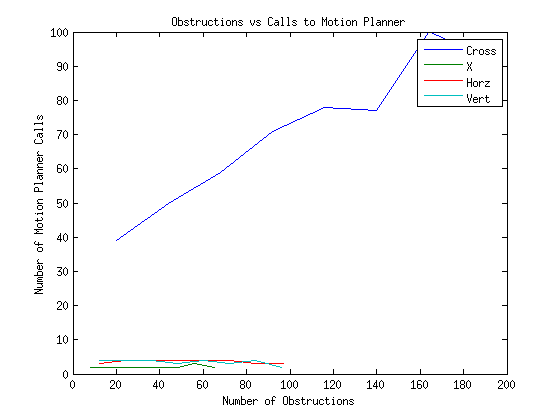
\includegraphics[width=.45\linewidth]{figures/ovm}}
	\qquad
	\subfloat{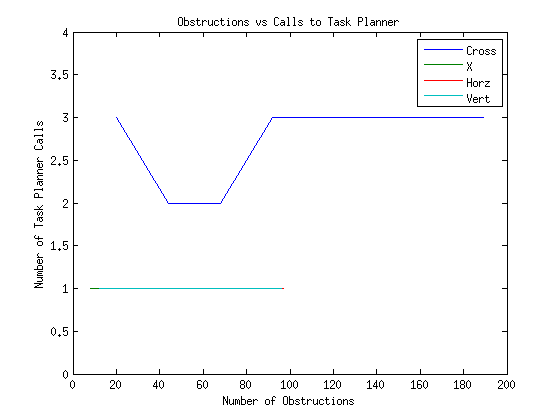
\includegraphics[width=.45\linewidth]{figures/ovt}}
	\qquad
	\subfloat{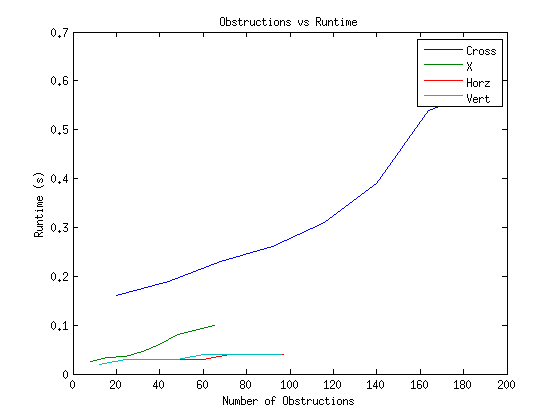
\includegraphics[width=.45\linewidth]{figures/ovrt}}
	\qquad
	\subfloat{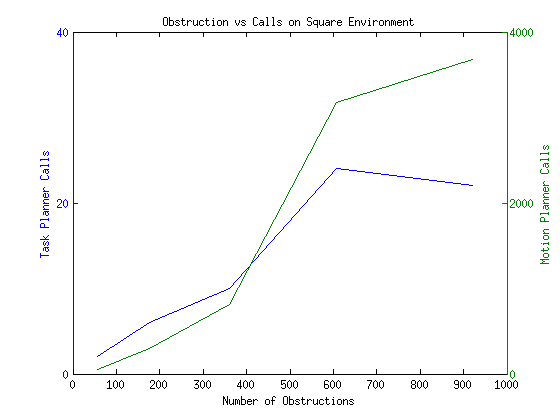
\includegraphics[width=.45\linewidth]{figures/square}}
	\caption{Benchmarking plots\label{fig:benchmarkPlots}}
\end{figure}
The goal of each test was to move the green block, at the center of a grid of blocks, to a goal surface. 
We tested a variety of different grid shapes, including a square grid, an X, a cross, and lines. 
We tested each grid shape over a range of sizes ranging from 3 to 13. ref{fig-benchmarks} 
The most difficult benchmark we tested was the 13x13 square grid. Larger tests caused the FF planner to segfault. As seen in \ref{fig:benchmarkPlots}, as the size of the problem increases the number of calls increases.

Figure \ref{benchmark2} shows the results for the original algorithm, minus our modification.  (Our modification always tries to find a perfect plan after adding a new high level plan section to the plan, rather than immediately trying to find a new partial trajectory.)  For the very simplest cases, the original algorithm performs better, since it makes the same number of motion and task planner calls but has less backtracking overhead.  However, for the more complicated environments, the cross and the square, our algorithm was significantly faster, as shown in \ref{benchmark}.

The interface layer is designed to be independent of any specific task and motion planner libraries, therefore number of calls to the motion and task planner measures the performance of the interface layer better than the total runtime, since the actual runtime will be very dependent on the motion planner and task planner chosen.

\begin{figure}
\begin{tabular}[t]{|l|l|l|l|l|l|}
\hline
Shape & Blocks & obstructions & Motion Planner Calls & Task Planner Calls & runtime \\ \hline
Horizontal Line & 3 & 12 & 3 & 1 & .023\\
& 5 & 24 & 4 & 1 & .028\\
& 7 & 36 & 4 & 1 & .029\\
& 9 & 48 & 4 & 1 & .029\\
& 11 & 60 & 4 & 1 & .034\\
& 13 & 72 & 4 & 1 & .037\\
\hline
Vertical Line & 3 & 12 & 4 & 1 & .024\\
& 5 & 24 & 4 & 1 & .027\\
& 7 & 36 & 4 & 1 & .028\\
& 9 & 48 & 4 & 1 & .028\\
& 11 & 60 & 4 & 1 & .037\\
& 13 & 72 & 4 & 1 & .036\\ 
\hline
X & 5 & 8 & 2 & 1 & .026\\
& 9 & 16 & 2 & 1 & .034\\
& 13 & 24 & 2 & 1 & .036\\
& 17 & 32 & 2 & 1 & .047\\
& 21 & 40 & 2 & 1 & .066\\
& 25 & 48 & 2 & 1 & .079\\ 
\hline
Cross & 5 & 20 & 39 & 3 & .16\\
& 9 & 44 & 50 & 2 & .20\\
& 13 & 68 & 59 & 2 & .23\\
& 17 & 92 & 71 & 3 & .26\\
& 21 & 116 & 78 & 3 & .31\\
& 25 & 140 & 77 & 3 & .39\\ 
\hline
Square & 9 & 56 & 54 & 2 & .16\\
& 25 & 176 & 294 & 6 & 1.06\\
& 49 & 360 & 818 & 10 & 5.07\\
& 81 & 608 & 3177 & 24 & 34.68\\
& 121 & 920 & 3681 & 22 & 87.06\\
& 169 & 1296 & 14216 & 57 & 518.61\\ 
\hline

\end {tabular}
\caption{Benchmark Tests - Our Modified Algorithm}
\label{benchmark}
\end{figure}


\begin{figure}
\begin{tabular}[t]{|l|l|l|l|l|l|}
\hline
Shape & Blocks & obstructions & Motion Planner Calls & Task Planner Calls & runtime \\ \hline
Horizontal Line & 3 & 12 & 3 & 1 & .016\\
& 9 & 48 & 4 & 1 & .025\\
& 13 & 72 & 4 & 1 & .033\\
\hline
Vertical Line & 3 & 12 & 4 & 1 & .022\\
& 9 & 48 & 4 & 1 & .027\\
& 13 & 72 & 4 & 1 & .031\\ 
\hline
X & 5 & 8 & 2 & 1 & .014\\
& 17 & 32 & 2 & 1 & .031\\
& 25 & 48 & 2 & 1 & .056\\ 
\hline
Cross & 5 & 20 & 47 & 5 & .15\\
& 17 & 92 & 206 & 10 & .68\\
& 25 & 140 & 390 & 14 & 1.56\\ 
\hline
Square & 9 & 56 & 145 & 11 & .45\\
& 25 & 176 & 4354 & 143 & 16.55\\

\hline

\end {tabular}
\caption{Benchmark Tests - Original Algorithm}
\label{benchmark2}
\end{figure}
\section{Limitations}

It is important to note that this planner is not guaranteed to find an optimal solution, or even to find a solution at all.  
We refer you to [1] for a proof that this algorithm is guaranteed to find a solution for problems with certain properties.  
However, due to the random nature of the pose generators and that there are limits set on the number of iterations, a valid plan may not be found for all problems.  

Furthermore, this system is not intended for online replanning.  
It may be possible to use it for online replanning for some systems if it runs quickly on the particular problem, but it is not an intended feature of this algorithm.

Finally, the runtime of this algorithm is based on the speed of the motion planner and the task planner used within it.  
If the motion planner and task planner are not efficient, the interface layer will not produce answers quickly.  
In particular, the number of calls to the motion planner is very large in order to gather the environmental information needed to pass on to the task planner.  
So in particular, the running time of this algorithm will depend on the running time of the motion planner.

\section{Open Questions}

The two immediately relevant open questions are whether it's possible to design a similar interface between task and motion plans which returns optimal plans or which can be used to do online planning.
Currently, the interface layer works only in deterministic, fully observable environments.  
It would be very interesting to develop similar algorithms to work in non-deterministic or partially observable environments as well.

Other interesting and relevant extensions could include the addition of more grasp primitives, for instance, push grasp primitives.




\section{References}

[1] S. Srivastava, E. Fang, L. Riano, R. Chitnis, S. Russell, P. Abbeel. "Combined Task and Motion Planning Through an Extensible Planner-Independent Interface Layer". IEEE International Conference on Robotics and Automation (ICRA), 2014.






\end{document}

